\chapter{Ionised Gas Distribution, Kinematics and Ionisation}
	\label{cha:gas}
The inter-stellar medium (ISM) in early-type galaxies (ETGs) has several components: a diffuse hot ($\sim 10^7 \, \mathrm{K}$) X-ray halo (with typical mass range $10^8$--$10^{10} \, \mathrm{M_\odot}$); warm ($\sim 10^4 \, \mathrm{K}$) ionised gas ($10^2$--$10^4 \, \mathrm{M_\odot}$), which can be more clumpy; and cold ($<10^2 \, \mathrm{K}$) atomic and molecular gas ($10^6$--$10^8 \, \mathrm{M_\odot}$), which generally confined to small (kpc or less) scale clouds. In this chapter we study the spatially resolved properties of the ionised gas component in radio galaxies (RGs) from the emission lines in the VIMOS and MUSE datacubes of the Southern Sample.

The chapter is structured as follows. First, the flux and equivalent width maps for each emission line within the relevant wavelength ranges of VIMOS and MUSE are shown. Gas masses are calculated and upper limits given in the cases of non-detections (see Section \ref{sec:GasFlux}). Secondly, in Section \ref{sec:GasKin}, the kinematics of the ionised gas is discussed. Finally, the source of the ionising potential is investigated, making use of several emission line diagnostics (see Section \ref{sec:Diagnostics}).


\section{Ionised Gas Fluxes}
	\label{sec:GasFlux}
	\subsection{Maps}
		\label{subsec:GasMaps}
		Only 4 galaxies of the Southern Sample have detections of emission lines outside of the central region (IC 1459, NGC 612, NGC 1316 and NGC 3100; see Figs.\,\ref{fig:VIMOS_Hb} and \ref{fig:MUSE_Hb}).  Of the remaining 7 galaxies, NGC 1399 has no detection of H$\beta$ at all, while the remaining 6 galaxies have detections only in the centre. 

		Images of each galaxy in the Southern Sample in H$\beta$ is shown in Figs.\ref{fig:VIMOS_Hb} and \ref{fig:MUSE_Hb}. All other emission lines have the same distribution, but at different intensities, with the exception of NGC 612, which shows a significant cloud in [\ion{O}{iii}] to the south of the centre of the galaxy (see Fig.\,\ref{fig:NGC612_OIII}). 


		\begin{figure}
			\centering
			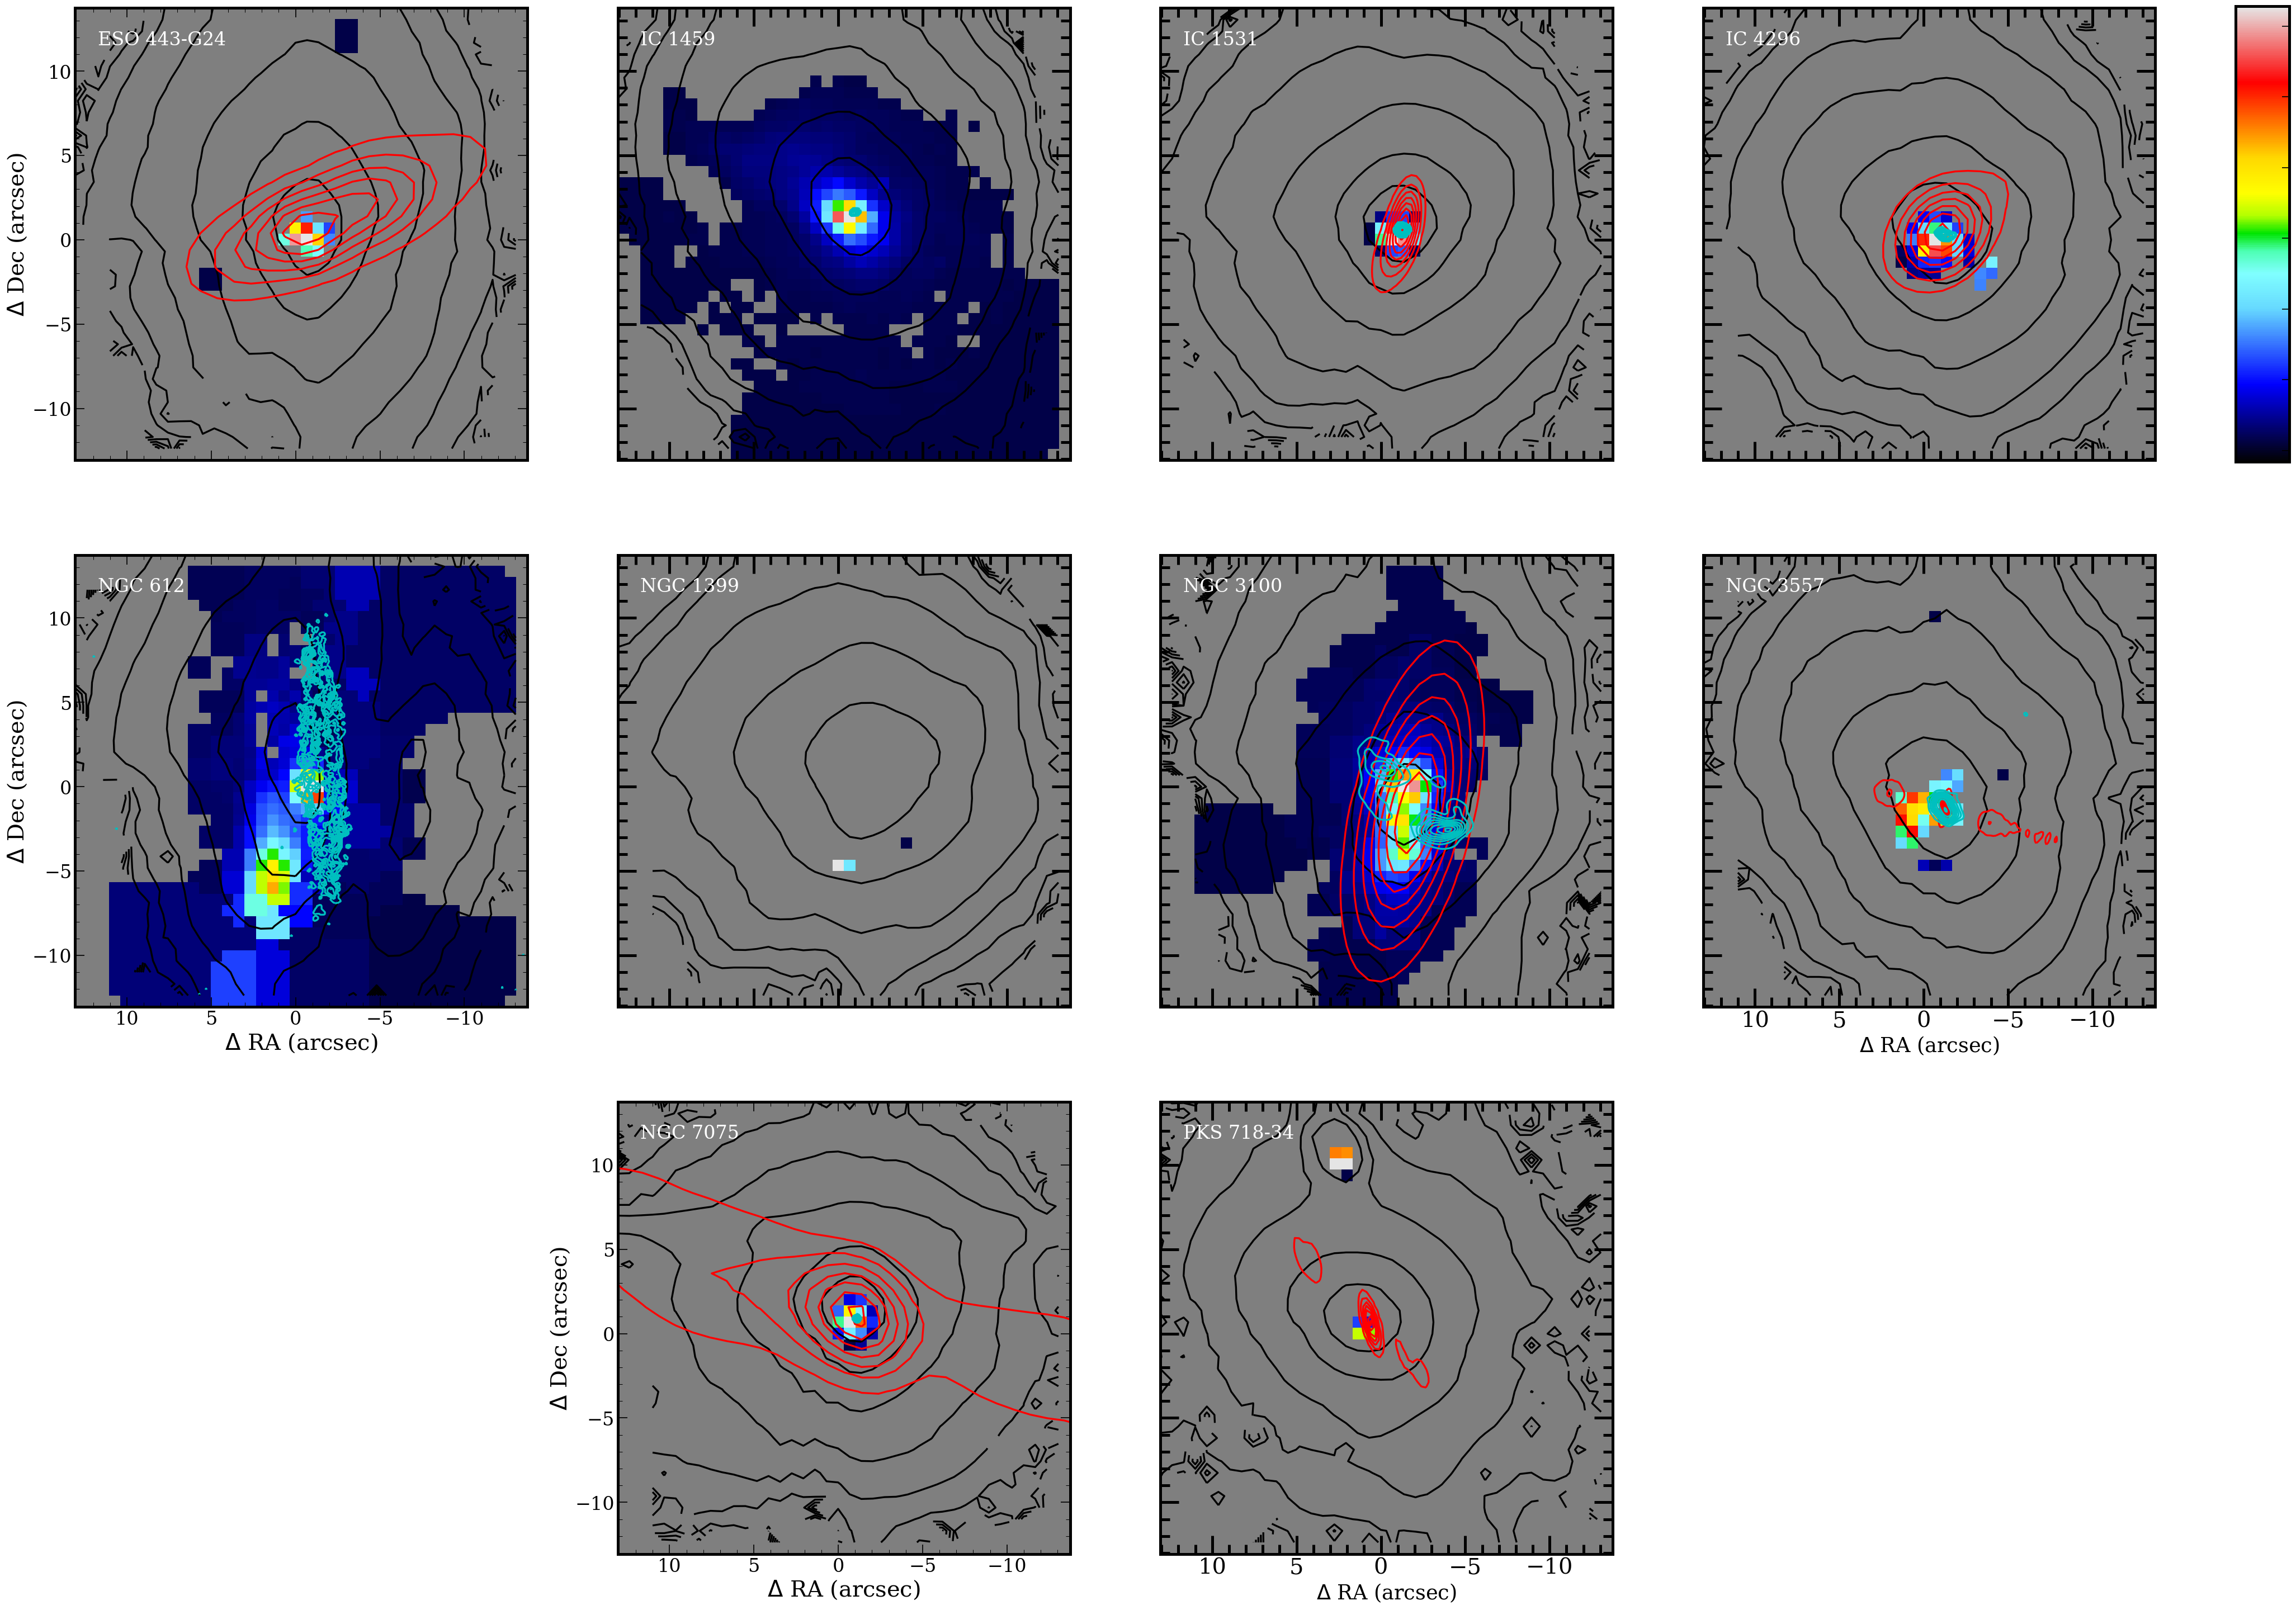
\includegraphics[width=\textwidth]{chapter5/vimos/Hb.png}
			\caption[VIMOS H$\beta$ maps]{VIMOS H$\beta$ maps.} 
			\label{fig:VIMOS_Hb}
		\end{figure}
		\begin{figure}
			\centering
			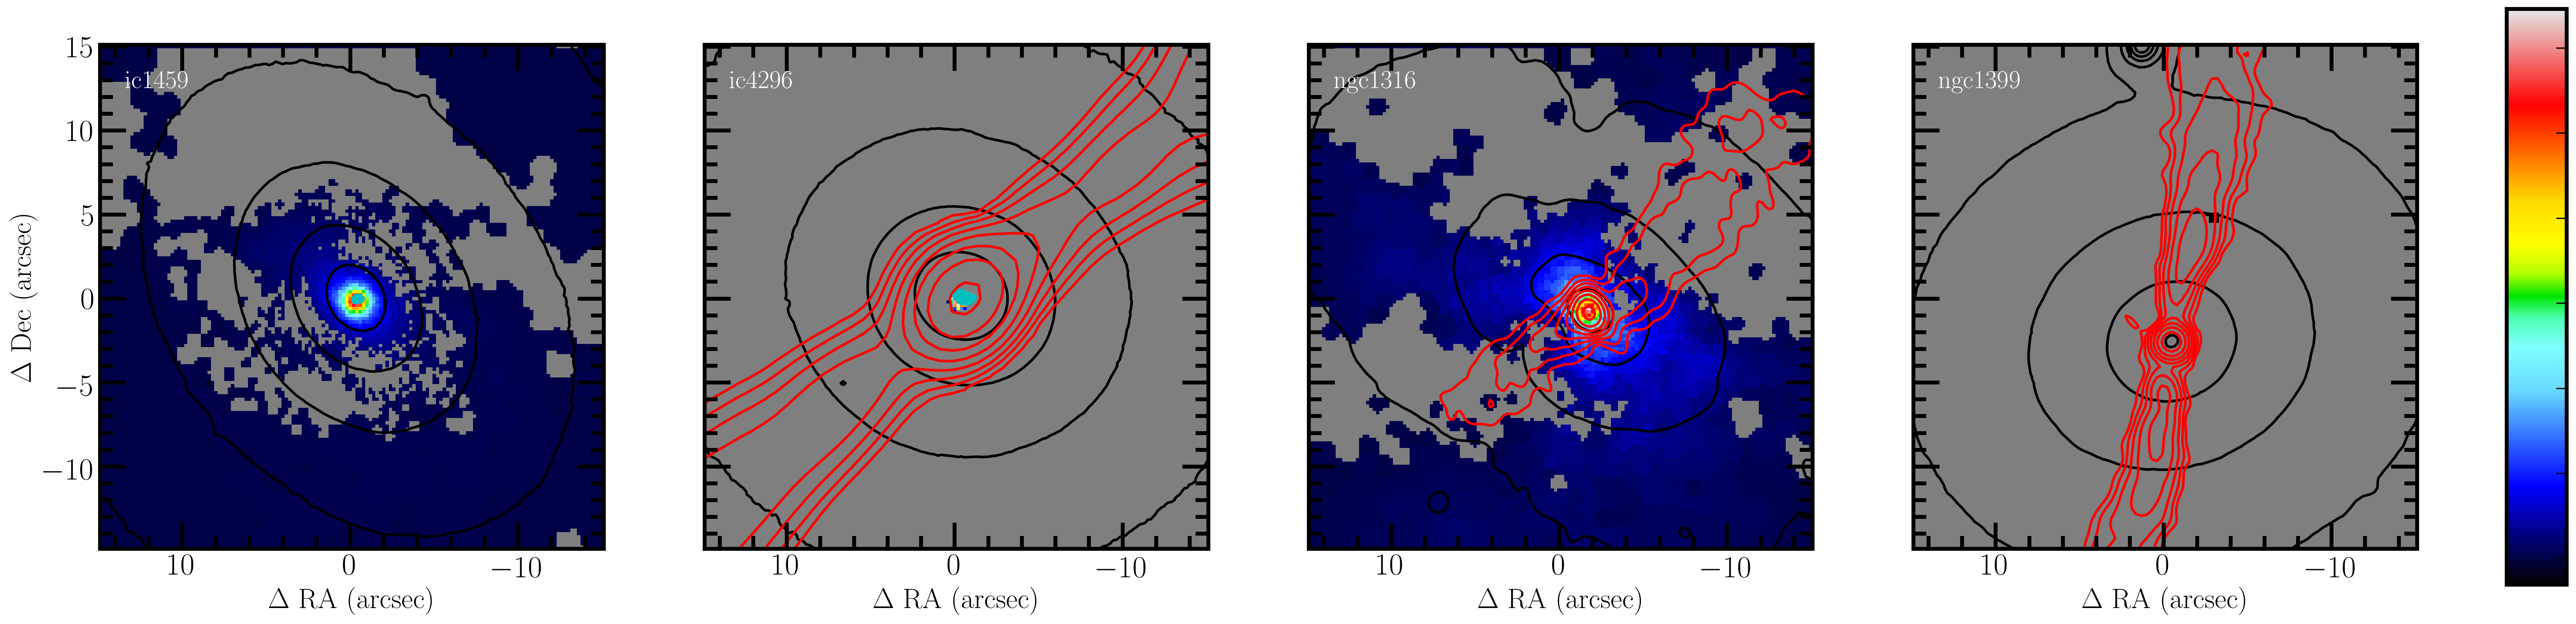
\includegraphics[width=\textwidth]{chapter5/muse/Hb.png}
			\caption[MUSE H$\beta$ maps]{MUSE H$\beta$ maps.} 
			\label{fig:MUSE_Hb}
		\end{figure}


		\begin{figure}
			\centering
			\includegraphics[width=0.4\textwidth]{chapter5/vimos/ngc0612_OIII_flux.png}
			\caption[NGC 612 \bracket{\ion{O}{iii}} image]{NGC 612 [\ion{O}{iii}] map showing a large cloud to the south of the centre of the galaxy, which is not present in the H$\beta$ map (see Fig.\ref{fig:VIMOS_Hb}).} 
			\label{fig:NGC612_OIII}
		\end{figure}


		Because equivalent width is not dependent on overall intensity (except for the initial detection threshold: a line must be detected in order to observe its equivalent width), it can be used to highlight local structures that cannot be seen in flux maps. The equivalent width maps for each emission line for each galaxy in the Southern Sample are shown in Figs.\,\ref{fig:VIMOS_ew} and \ref{fig:MUSE_ew}. 

		\begin{figure}
			\centering
			\includegraphics[width=\textwidth]{chapter5/vimos/ew.png}
			\caption[VIMOS equivalent width maps]{VIMOS equivalent width maps.} 
			\label{fig:VIMOS_ew}
		\end{figure}
		\begin{figure}
			\centering
			\includegraphics[width=\textwidth]{chapter5/muse/ew.png}
			\caption[MUSE equivalent width maps]{MUSE equivalent width maps.} 
			\label{fig:MUSE_ew}
		\end{figure}

	\subsection{Gas Masses}
		\label{subsec:GasMass}

		Gas masses are derived using the recipe from \citet{Sarzi2005}. This is very rough calculation and the values should not be used for quantitative applications. The approach follows \citet{Kim1989}, and as such
		\begin{equation}
			M_\text{\ion{H}{ii}} = 280 \left(\frac{D}{10\, \mathrm{Mpc}}\right)^2 \frac{F(\mathrm{H\alpha})}{10^{-14} \, \mathrm{erg \, s^{-1} \, cm^{-2}}} \frac{10^3 \, \mathrm{cm^{-3}}}{n_\mathrm{e}} \, ,
		\end{equation}
		where $M_\text{\ion{H}{ii}}$ is the mass in solar mass ($M_\odot$) of \ion{H}{ii} in a galaxy $D$ Mpc away, with an observed H$\alpha$ flux of $F(\mathrm{H\alpha})$. The electron density is assumed to be, $n_\mathrm{e} = 100 \, \mathrm{cm^{-3}}$. 
		% This method assumes B-type recombination and a temperature of 10^4 K.
		Like \citet{Sarzi2005}, we only claim a detection if the amplitude-to-noise ratio (A/N) is $>4$ for [\ion{O}{iii}] and $>2.5$ for H$\beta$. Since most of the gas is centrally concentrated using a large field of view, often only serves to increase the noise (reducing A/N). Our lower limits on the gas mass, are set by the mass measured from the largest aperture that still meets our detection criteria. This would be the gas mass of the galaxy if there was no gas at larger radii. Upper limits are set by the mass found from the H$\alpha$ flux increased by one $\sigma$ for the entire field of view (i.e. $F(\mathrm{H\alpha})+\delta F(\mathrm{H\alpha})$ is used). If a detection is found for the entire field of view, then Table \ref{tab:gasMass} the upper and lower limit columns are combined to show a single value. 


		\begin{table}
			\centering
		\begin{threeparttable}
			\caption{Gas Masses for the Southern Sample.}
			\label{tab:gasMass}
			\begin{tabular*}{0.8\textwidth}{@{\extracolsep{\fill}}l r r r}
				\hline
				\hline
				Galaxy & VIMOS \ion{H}{ii} Mass & MUSE \ion{H}{ii} Mass & Balmer Decrement \\
				& \multicolumn{1}{c}{$[\mathrm{M_\odot}]$} & \multicolumn{1}{c}{$[\mathrm{M_\odot}]$} & \\
				\hline
				ESO 443-G024 & $5.27 \pm 0.01$ 	& --  		& -- \\
				IC 1459 	& $5.38 \pm 0.01$	& $5.36 \pm 0.01$ & $3.61 \pm 0.04$ \\
				IC 1531 	& $5.70 \pm 0.01$	& -- 		& -- \\
				IC 4296		& $5.16 \pm 0.01$	& $5.08 \pm 0.01$ & --\tnote{a} \\
				NGC 612 	&  		& -- 		& -- \\
				NGC 1316 	& -- 		& $-2.52 \pm 0.01$ & $4.12 \pm 0.06$ \\
				NGC 1399 	& $<$ 	& $-3.88 \pm 0.01$ & $<30$\tnote{b} \\
				NGC 3100 	&  		& -- 		& -- \\
				NGC 3557 	&  		& -- 		& -- \\
				NGC 7075 	&  		& -- 		& -- \\
				PKS 718-34  &  		& -- 		& -- \\
				\hline
				\hline
			\end{tabular*}
			\begin{tablenotes}
			\footnotesize
			\note Col.\,1: Galaxy. Col.\,2: \ion{H}{ii} mass derived from the H\,$\beta$ line in the VIMOS data, assuming a Balmer decrement of 2.85. Col.\,3: \ion{H}{ii} mass derived from the H\,$\alpha$ line in the MUSE data. Col.\,4: Observed Balmer decrement derived from the MUSE data.
			\item [a] H$\beta$ was not detected in IC 4296, thus the formal observed Balmer decrement is $\infty$. 
			\item [b] H$\beta$ was not detected with an A/N $> 2.5$ meaning that the fit is not reliable (hence this is an upper limit). 
			\end{tablenotes}
		\end{threeparttable}
		\end{table}
		









\section{Ionised Gas Kinematics}
	\label{sec:GasKin}
	Using the methods described in Section \ref{subsec:EmissionFit} we find the best-fitting line-of-sight velocity distribution (LOSVD; assumed to be Gaussian in form and represented by the mean velocity and velocity dispersion only) for the ISM. As described in \ref{subsec:EmissionFit}, all emission lines are fitted with the same LOSVD, but with each individual line fitted with its own flux. In the cases of the [\ion{O}{iii}], [\ion{O{i}}] and [\ion{N}{ii}] doublets, the components of the doublets are fitted with a fixed flux ratio of 1:0.34; the [\ion{N}{i}] doublet has a ratio of 1:0.65 \citep{Safier1992}; and the components of the [\ion{O}{ii}] and [\ion{S}{ii}] doublets are fitted independently.

	In Figs.\,\ref{fig:VIMOS_Gaskine} and \ref{fig:MUSE_Gaskine}, we show the maps of the mean velocity and velocity dispersion for the ISM in the galaxies with a significant number of spatial bins that have gas detected in our Southern sample (IC 1459, NGC 612, NGC 1316 and NGC 3100). 

	\begin{figure}
		\centering
		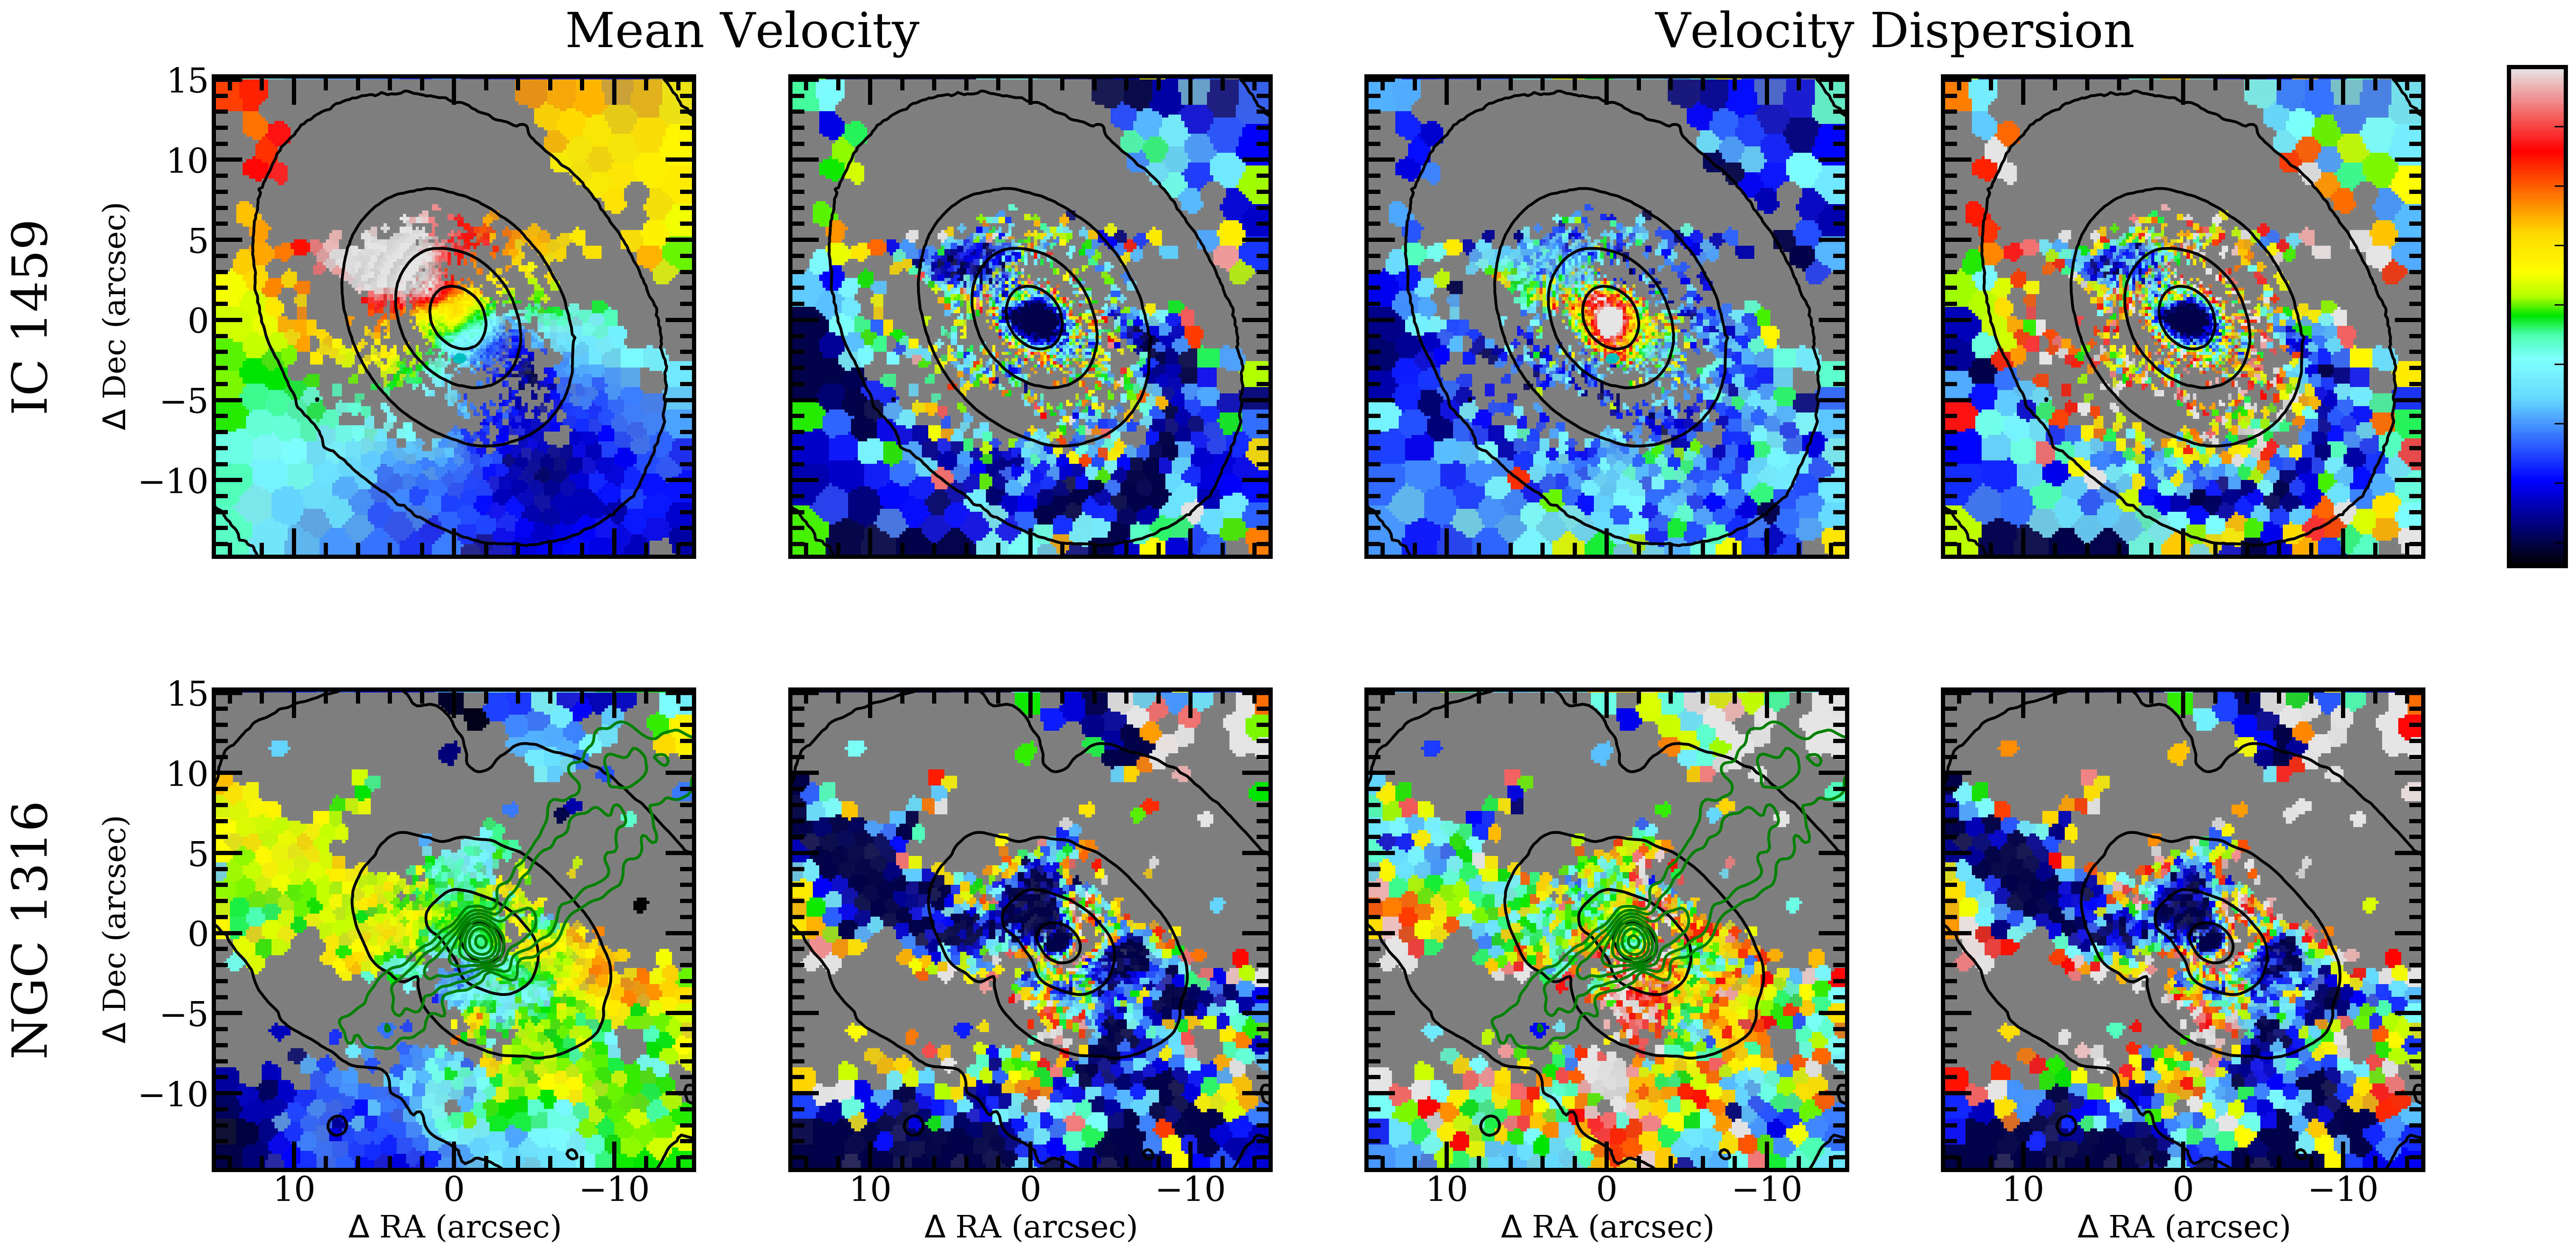
\includegraphics[height=0.62\textheight]{chapter4/vimos/kin.png}
		\caption[VIMOS ISM kinematic maps]{VIMOS ISM kinematic maps. Left to right: mean velocity and velocity dispersion. Alternate columns show a given parameter its associated uncertainty. Top to bottom: IC 1459, NGC 612 and NGC 3100. Flux contours (isophotes) are shown in black, \ce{^{12}CO(2-1)} contours from ALMA in cyan and radio continuum contours from VLA in green. The radio band displayed depends on the data available in the archive and which images had a similar resolution and scales. Limits on the colour scale are: mean velocity maps -360 to 360\,$\mathrm{km \, s^{-1}}$ (except for NGC 3100 which has limits of -100 to 100\,$\mathrm{km \, s^{-1}}$), mean velocity uncertainty 1 to 15\,$\mathrm{km \, s^{-1}}$, velocity dispersion 35 to 200\,$\mathrm{km \, s^{-1}}$ and velocity dispersion uncertainty 1 to 20\,$\mathrm{km \, s^{-1}}$.} 
		\label{fig:VIMOS_Gaskine}
	\end{figure}

	\begin{figure}
		\centering
		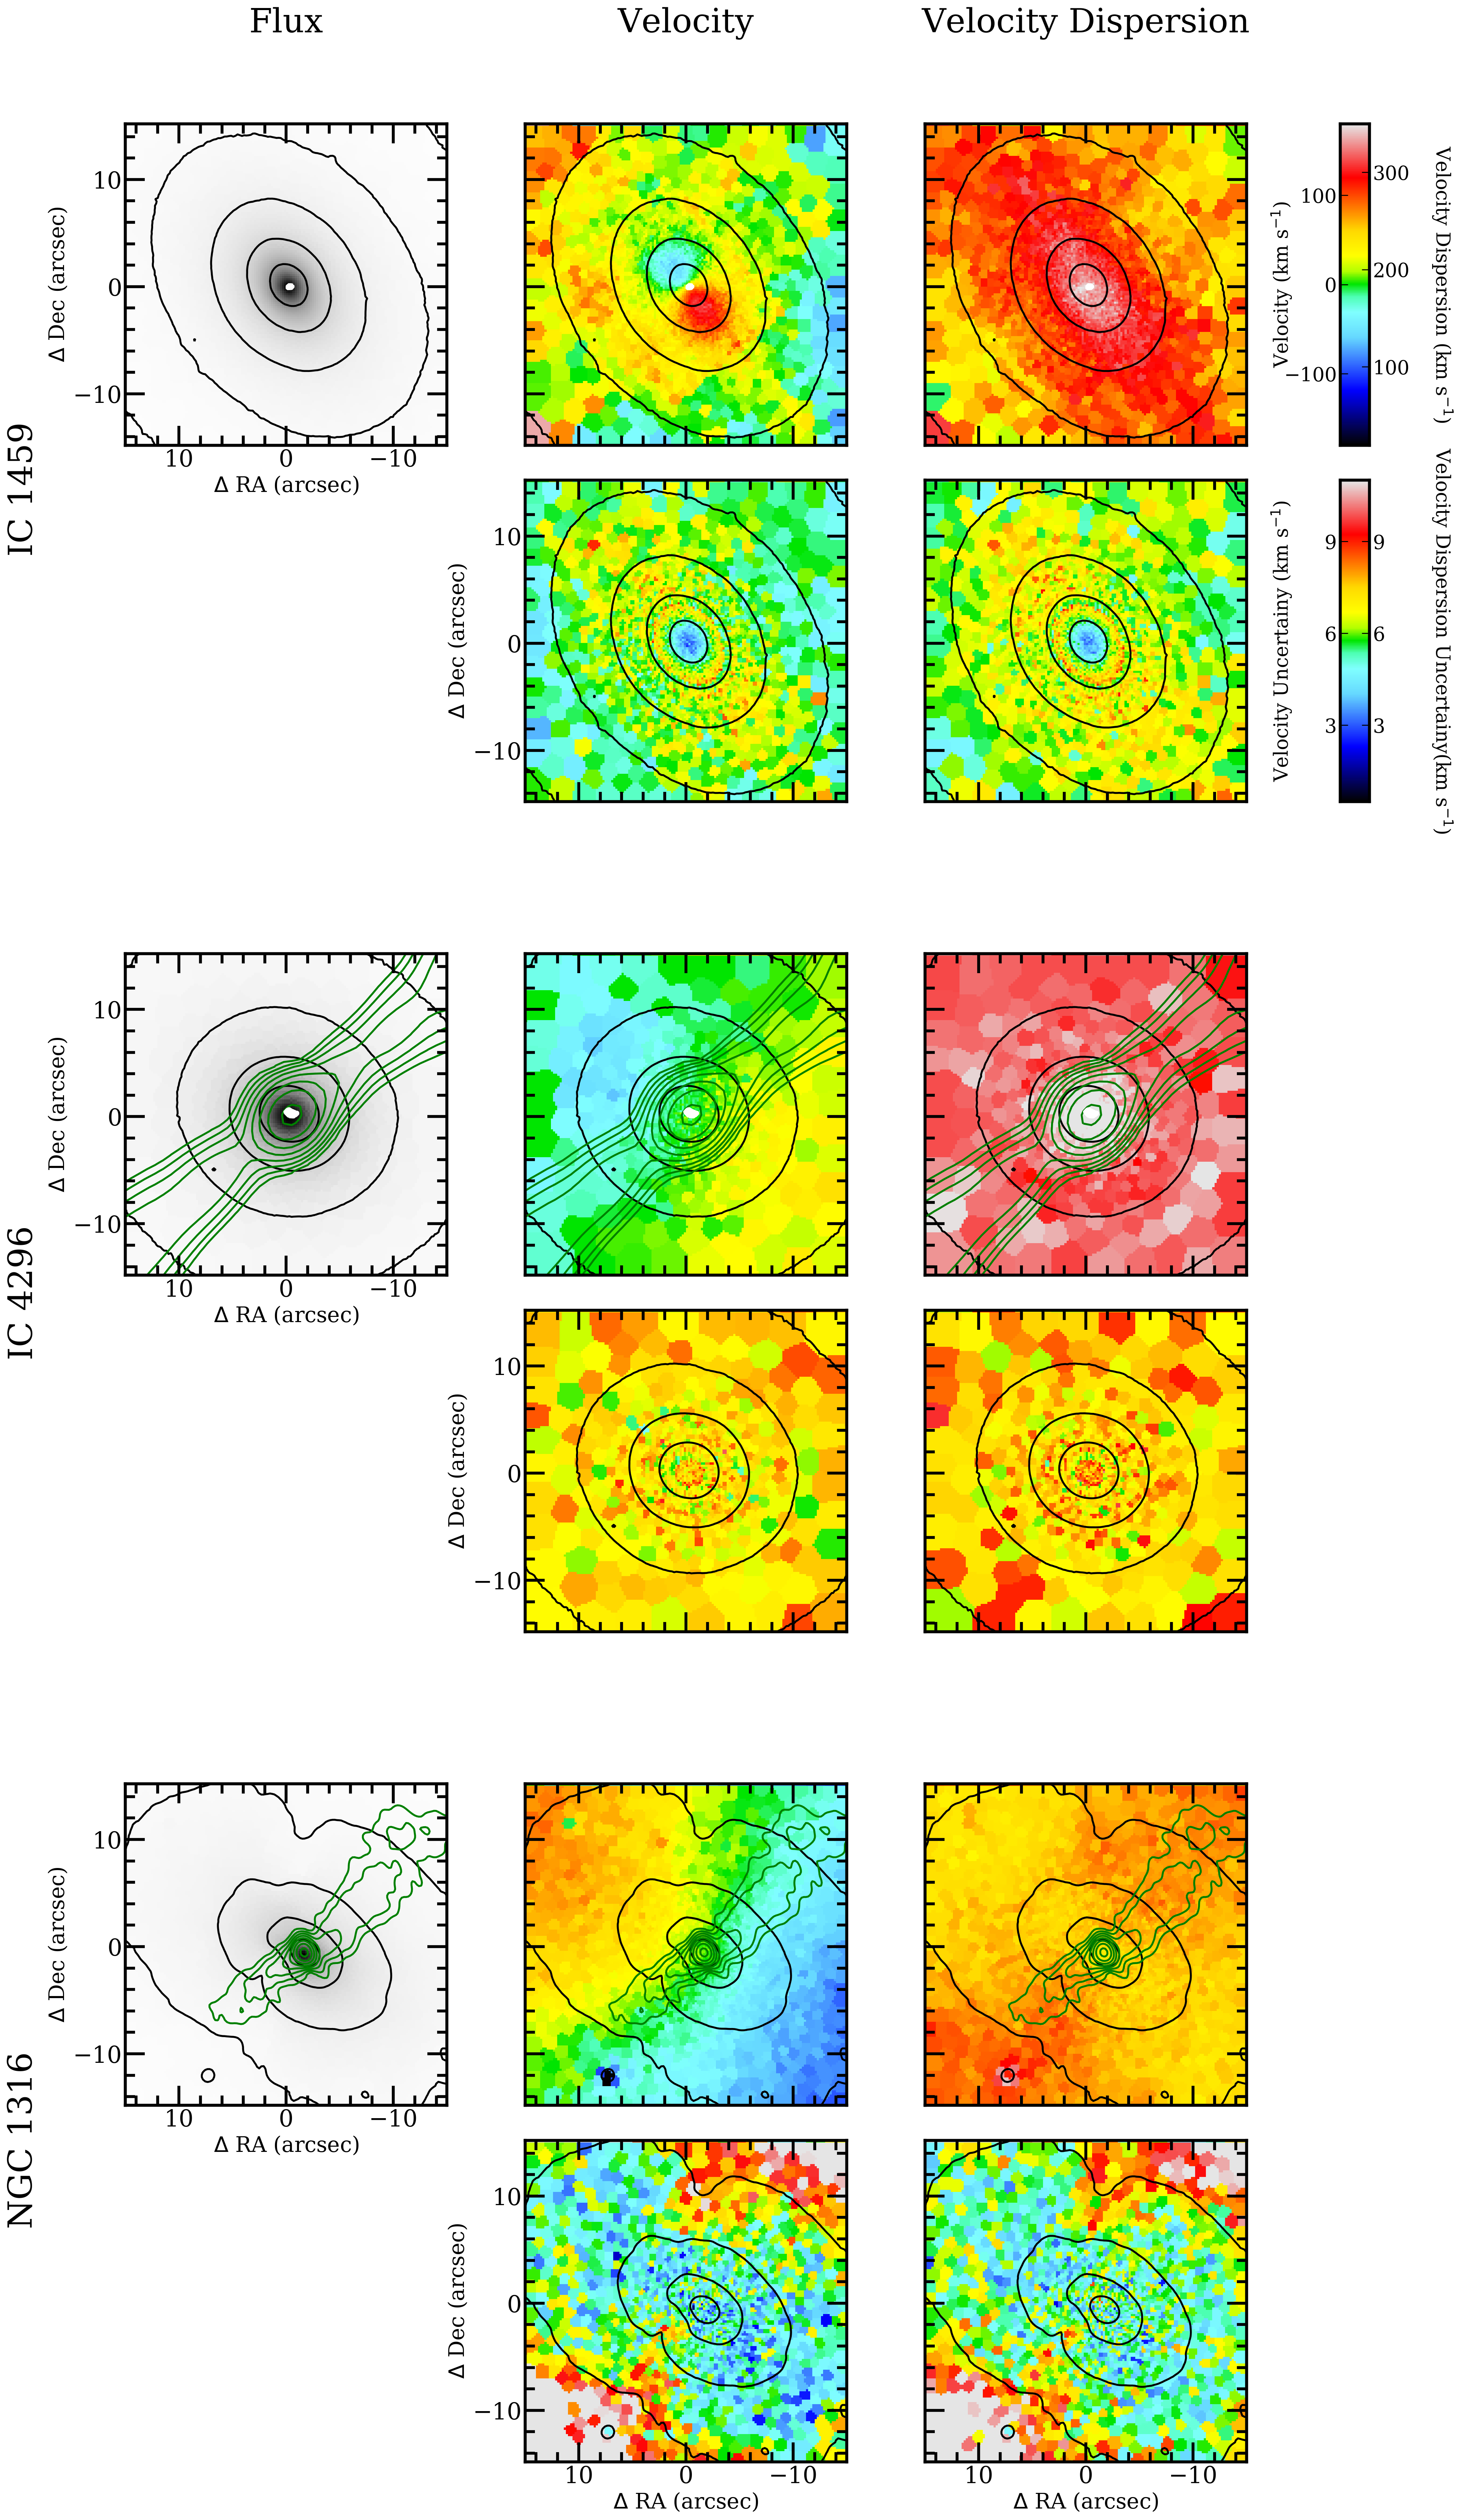
\includegraphics[height=0.94\textheight]{chapter4/muse/kin1.png}
		\caption[MUSE ISM kinematic maps]{As in Figure \ref{fig:VIMOS_Gaskine} but for the MUSE ISM kinematic maps.}
		\label{fig:MUSE_Gaskine}
	\end{figure}












	\subsection{Misalignment of Gas}
		\label{subsec:Gasmisaligment}
		It is immediately clear when comparing the mean stellar velocity maps in Figs.\,\ref{fig:VIMOS_stellar} and \ref{fig:MUSE_stellar} to the mean gas velocity maps in Figs.\,\ref{fig:VIMOS_gaskine} and \ref{fig:MUSE_gaskine} that where gas is detected, its angular momentum vector is not often aligned with that of the stars. IC 1459 shows the gas counter-rotating with respect to the kinematically-decoupled core, and rotating independently from the rest of the galaxy too. The kinematics of the gas in NGC 612 appear to be well aligned to that of the stars. 




	\subsection{The Changing Orbits of the ISM}
		\label{subsec:outflows}

































\section{Sources of Ionising Potential}
	\label{sec:Diagnostics}
	Determining the source of the ionising radiation using line ratio plots, such as Baldwin--Phillips--Terlevich (BPT) diagrams (\citealt{Baldwin1981}; and revised by \citealt{Kewley2001, Kauffmann2003a}), has become increasingly useful tool. That said, there are several important caveats. Firstly, great care must be taken in applying the definitions of each diagnostics line. Much of the literature mis-interprets the classifications. Secondly, in the absence of spatially resolved spectra, low-ionisation nuclear emission-line region (LINER) classifications have often been taken as a marker for jet-mode active galactic nuclei (AGN). As discussed in Section \ref{subsubsection:JetFeedback}, several recent surveys have shown that many of these galaxies may not be bona fide AGN \citep[e.g.][]{Sarzi2005, Sarzi2010, Singh2013, Belfiore2016a}. In such cases, the emission may not even originate from the centre of the galaxies, the location of the supposed AGN. This led to the creation of the low-ionisation emission-line region (LIER) classification, with the same criteria as LINER, but not necessarily in the nuclear region.

	This section is laid out as follows. Firstly we find the conversion factors from [\ion{N}{ii}] to [\ion{N}{i}] and [\ion{O}{i}] to [\ion{O}{iii}] (Section \ref{subsec:Ndec}). With the Balmer decrement, this allows the use of diagnostic plots that use either H$\alpha$, [\ion{N}{ii}] or [\ion{O}{i}] emission lines, for data where these emission lines are outside of the wavelength range i.e. we use [\ion{N}{i}], [\ion{O}{iii}] and H$\beta$ as proxies for [\ion{N}{ii}], [\ion{O}{i}] and H$\alpha$ respectively. We then examine each of the the following diagnostics plots for each galaxy: BPT plots, mass--excitation (MEx), equivalent width of H$\alpha$ verse [\ion{N}{ii}]/H$\alpha$ line ratio (WHaN2).%; or for VIMOS, the equivalent width of H$\beta$ verse [\ion{N}{i}]/H$\beta$ line ratio i.e. WHbN1). 

	% \subsection{\bracket{\ion{N}{ii}} to \bracket{\ion{N{i}}} Ratio in MUSE Data}
	\subsection{Using Emission Lines Beyond the Range of VIMOS Data}
		\label{subsec:Ndec}

		The Balmer decrement, $d_\mathrm{H}$, is the ratio of the H$\alpha$ to H$\beta$ fluxes and has good theoretical motivation that it has a near constant value of $d_\mathrm{H} = 2.86$ under a wide variety of conditions. In reality, however, higher values are routinely observed. These observation can be explained as either due to the presence of dust, causing extinction, whereby emission lines at longer wavelengths to appear brighter than expected compared the their bluer counterparts as the dust preferentially scatters bluer light; or some mechanism that populates hydrogen levels from the ground up. Such mechanisms may be important in high-density environments such at within powerful (type 1) AGN nuclei \citep[e.g.][]{Shields1974, Netzer1975}. The majority ($\approx 60$\%) of ETGs and all low-ionized nuclear emission region galaxies (LINERs) and Seyfert galaxies are dusty in nature \citep[e.g.][]{Martini2013}. Such galaxies have clear dust observations in \textit{Hubble Space Telescope (HST)} observations \citep[e.g.][]{Martini2013}, are bright in the infrared (where the thermal emission from dust is seen in the `dust bump'; e.g. \citealt{Jura1987, Knapp1992}) and other emission line ratios \citep[e.g. \bracket{\ion{S}{ii}} in ][]{Wampler1968} show similar reddening. Thus, assuming the observed steeping of the Balmer decrement is entirely due to dust, the ratio of the observed decrement to the theoretical value of 2.86 is a good estimate for the reddening effect of the dust.

		If we assume that different ionization states of a given atom occur in the same locations (namely, the location of the abundance of the atom), implying that shielding is not important or at least is not non-linear in its affect on the emission-line ratios. Given that the different species must have been produced under the same conditions, it might be natural to expect a relationship between them. Thus, using the emission line fluxes derived from the MUSE data, we observe that the relationship between [\ion{N}{ii}] and [\ion{N}{i}] appears to be linear, while the relationship between [\ion{O}{i}] and [\ion{O}{iii}] appears to be quadratic. We emphasis that these are purely empirical observations and differ from the Balmer decrement as they lack strong theoretical basis. 

		In order find the intrinsic conversion from both [\ion{O}{iii}] and [\ion{N}{i}] to [\ion{O}{i}] and [\ion{N}{ii}] we must first correct them for dust reddening. Assuming that the extinction can be approximated to a linear form in the V-band, we correct the flux of the bluer emission line, $I_\mathrm{b}$ of the pair by applying
		\begin{equation}
			I^\mathrm{corr}_\mathrm{b} = I_\mathrm{b} \frac{\Delta\lambda}{\lambda_\mathrm{H\alpha} - \lambda_\mathrm{H\beta}} \frac{I_\mathrm{H\alpha}}{2.86 I_\mathrm{H\beta}} \, ,
		\end{equation}
		where $\Delta\lambda$ is the difference in wavelength of the two lines, $\lambda_\mathrm{H\alpha}$ and $\lambda_\mathrm{H\beta}$ are the rest-frame wavelengths of the H$\alpha$ (6563 \AA) and H$\beta$ (4861 \AA) emission lines with intensities of $I_\mathrm{H\alpha}$ and $I_\mathrm{H\beta}$, respectively. The intrinsic conversion can then be found by comparing $I^\mathrm{corr}_\mathrm{b}$ to $I_\mathrm{r}$, the intensity of the redder line in the pair. 

		In Fig.\,\ref{fig:NII_NI} we fit a straight line to the intensity of [\ion{N}{ii}] verse [\ion{N}{i}] corrected for dust extinction using the least-trimmed squares routine, \textsc{lts\_linefit} by \citet{Cappellari2013} due to its robust handling of uncertainty in both axes. In Fig.\,\ref{fig:OI_OIII} we fit a quadratic to the intensity of [\ion{O}{i}] verse [\ion{O}{iii}] corrected for dust extinction. For this fit with use the orthogonal distance regression routines (ODR) within the \textsc{scipy} package. ODR must be used with care, particularly when the functional form of the model is not well known, i.e. the residuals to the fit may not be purely noise. While this is the case here: we have no theoretical reason for fitting a quadratic, we can see from Fig.\,\ref{fig:OI_OIII} that it is a good fit across 8 orders of magnitude in the [\ion{O}{iii}] direction. Thus, while, the actual parameters of the fit may not reflect the underlying physics, they do give a good representation of the data.

		In this way, we find the following relationships:
		\begin{align}
			I_\text{[\ion{N}{ii}]} = & \, a I^\text{corr}_\text{[\ion{N}{i}]} + b \\
			\intertext{and}
			I_\text{[\ion{O}{i}]} = & \, (8.02 \pm 0.43) \times 10^{-6} I^\text{corr}_\text{[\ion{O}{iii}]}^2 + (0.388 \pm 0.009) I^\text{corr}_\text{[\ion{O}{iii}]} + (1.37 \pm 0.11) \times 10^{-6} \, .
		\end{align}


		\begin{figure}
			\centering
			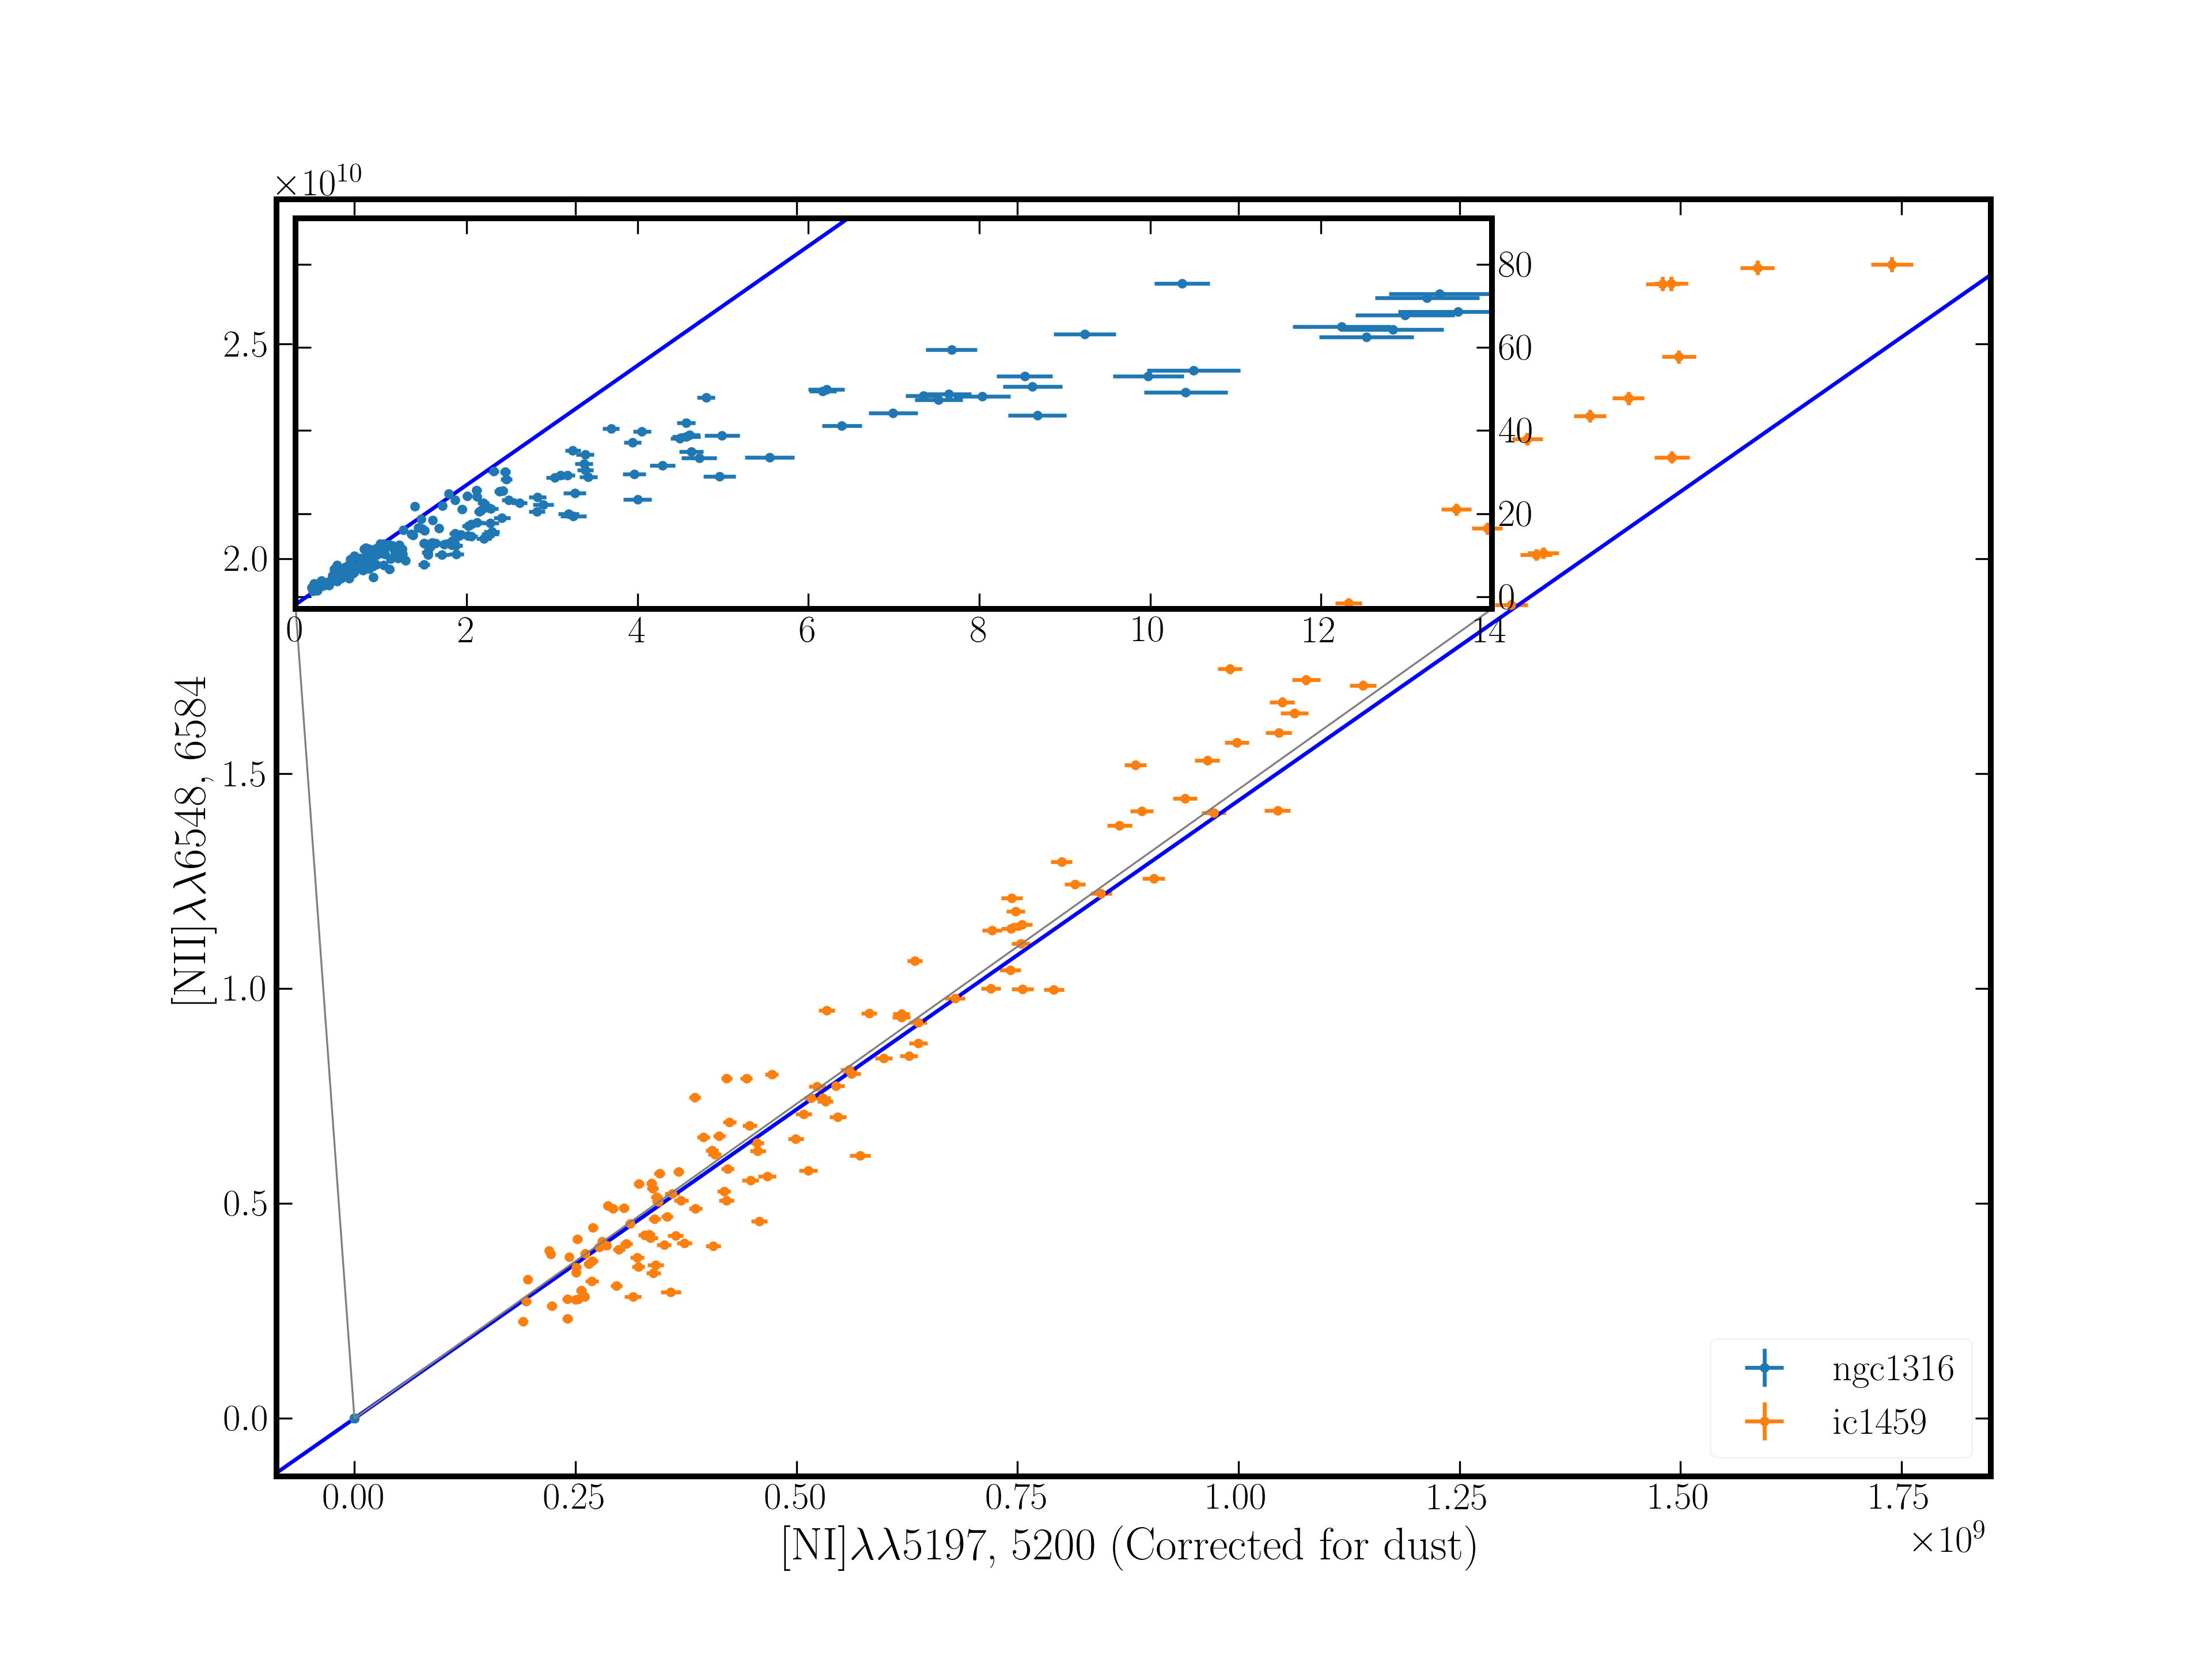
\includegraphics[width=\textwidth]{chapter5/vimos/NII_NI_ratio.png}
			\caption[The nitrogen `decrement']{The Nitrogen `decrement'.} 
			\label{fig:NII_NI}
		\end{figure}

		\begin{figure}
			\centering
			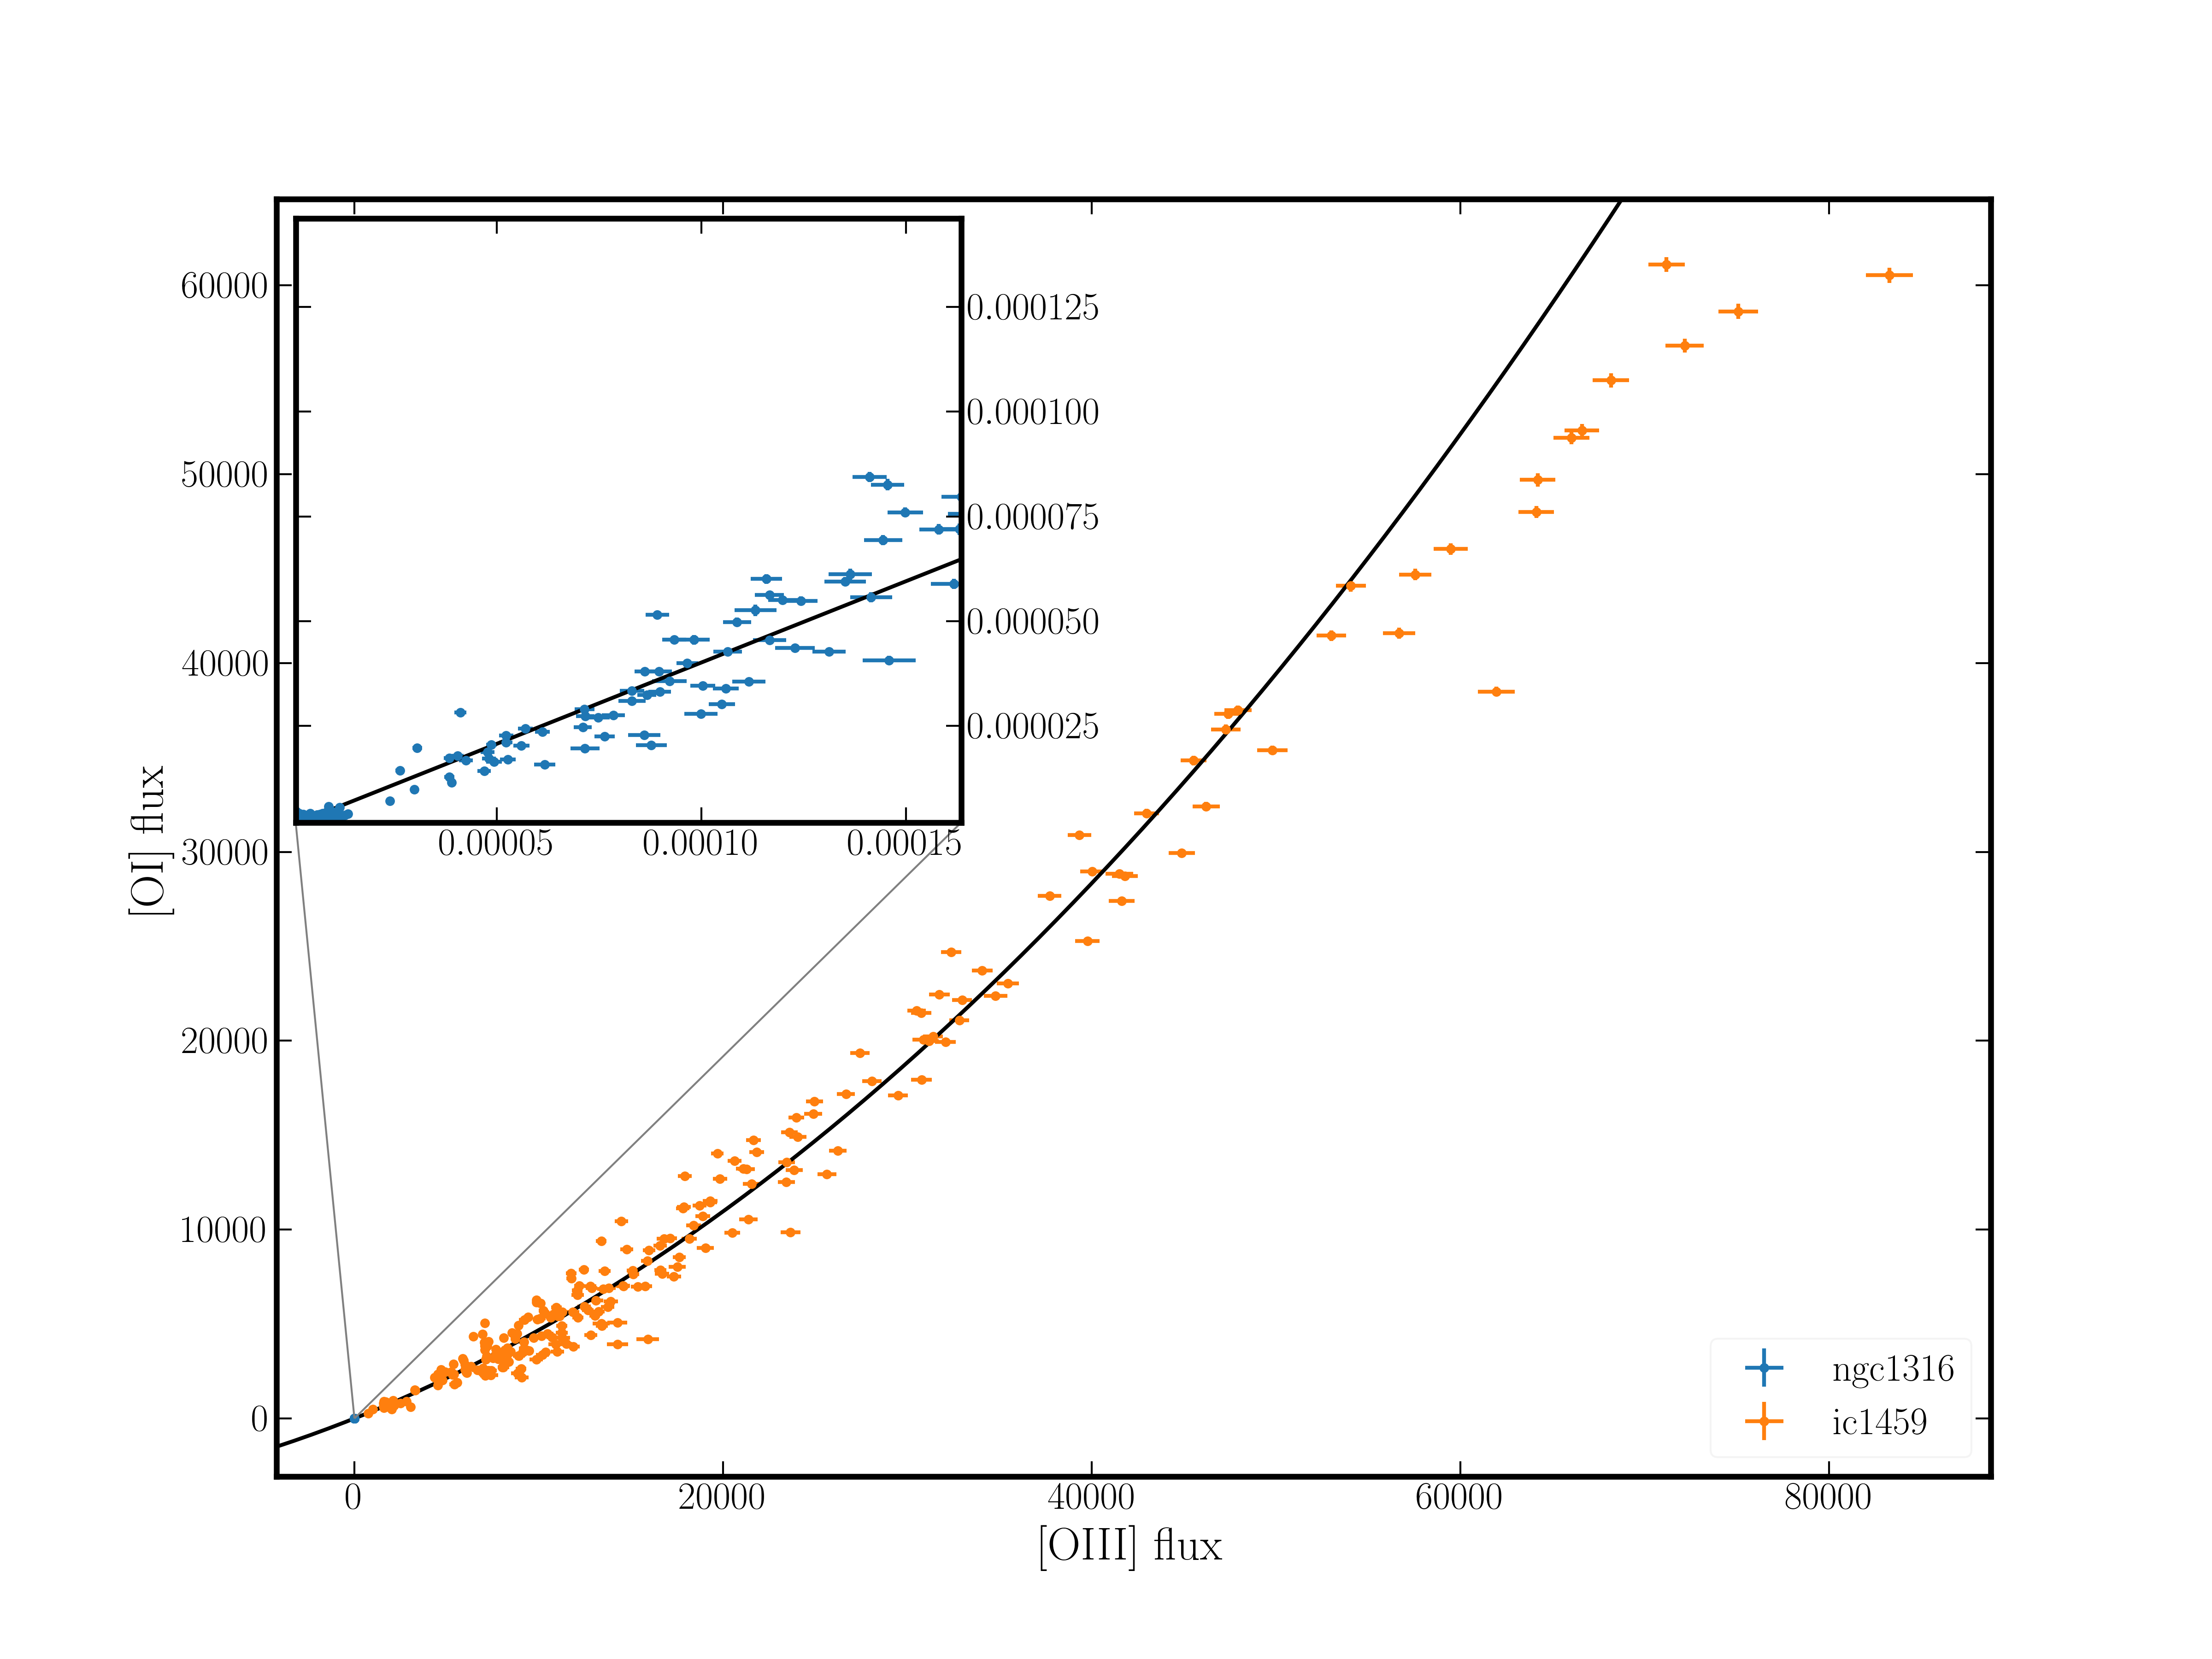
\includegraphics[width=\textwidth]{chapter5/OIII_OI_ratio.png}
			\caption[The oxygen `decrement']{The oxygen `decrement'.} 
			\label{fig:OI_OIII}
		\end{figure}



		Since H$\alpha$, [\ion{O}{i}] and [\ion{N}{ii}] emission lines are all outside of the wavelength range of VIMOS, we transpose observations and empirical boundary lines  
%Need a better description of the lines
		using the Balmer decrement, a linear fit to an analogous `nitrogen decrement' and a quadratic fit to the `oxygen decrement'.

	\subsection{BPT Diagnostic Plots}
		\label{subsec:BPT}
% Include SUARON diagnoistic plots here


	\subsection{MEx Diagnostic Plots}
		\label{subsec:MEx}


	\subsection{WHaN2 Plots}
		\label{subsec:WHaN2}


